\documentclass[11pt,a4paper]{ctexart}

% =====================================================
% 高中数学问题解决方法论 · 学生手册 v2
% 设计原则：先建立统一决策框架，再挂载具体方法与专题工具
% =====================================================

% ---------- 优先使用项目既有 ipara 样式；缺失时启用独立预览样式 ----------
\newif\ifipara
\IfFileExists{ipara.sty}{%
  \iparatrue
  \usepackage[student]{ipara}
}{%
  \IfFileExists{common/ipara.sty}{%
    \iparatrue
    \usepackage[student]{common/ipara}
  }{\iparafalse}
}

\ifipara\else
  \usepackage{geometry}
  \geometry{left=1.7cm,right=1.7cm,top=2.0cm,bottom=2.0cm}
  \usepackage{xcolor}
  \usepackage{amsmath,amssymb,mathtools}
  \usepackage{booktabs,tabularx,array}
  \usepackage[most]{tcolorbox}
  \usepackage{enumitem}
  \setlist{nosep,leftmargin=2em}
  \definecolor{rulecolor}{gray}{0.25}
  \newtcolorbox{lessonbriefbox}[1]{
    breakable,colback=white,colframe=black!65,boxrule=0.7pt,
    title=\textbf{#1},fonttitle=\bfseries,arc=1mm,left=1.2mm,right=1.2mm}
  \newtcolorbox{theorembox}[1]{
    breakable,colback=black!2,colframe=black!55,boxrule=0.7pt,
    title=\textbf{#1},fonttitle=\bfseries,arc=1mm}
  \newtcolorbox{keybox}[1]{
    breakable,colback=black!4,colframe=black!75,boxrule=0.9pt,
    title=\textbf{#1},fonttitle=\bfseries,arc=1mm}
  \newcommand{\mindsetcard}[3]{%
    \begin{tcolorbox}[breakable,colback=white,colframe=black!70,boxrule=0.8pt,arc=1mm]
    {\large\bfseries #1}\hfill{\small\bfseries #2}\par\smallskip
    #3
    \end{tcolorbox}}
  \newcommand{\problemheader}[1]{\par\medskip\noindent{\large\bfseries #1}\par\smallskip}
  \newcommand{\answerblank}[2][3cm]{\noindent #2\par\vspace{#1}}
  \newcommand{\checkbox}{$\square$}
  \newcommand{\postproblem}[3]{%
    \begin{tcolorbox}[breakable,colback=black!1,colframe=black!35,title=复盘]
    \textbf{思考提示}\begin{itemize}#1\end{itemize}
    \textbf{完成检查}\par #2\par\vspace{#3}
    \end{tcolorbox}}
  \newcommand{\sidefigureproblem}[3]{%
    \begin{minipage}[t]{#1\linewidth}#2\end{minipage}\hfill
    \begin{minipage}[t]{\dimexpr\linewidth-#1\linewidth-0.03\linewidth\relax}\centering #3\end{minipage}}
\fi

% ---------- 本文件额外依赖 ----------
\usepackage{longtable}
\usepackage{tikz}
\usepackage{tikz-3dplot}
\usetikzlibrary{shapes.geometric,arrows.meta,positioning,calc,fit}
\usepackage{amsthm}
\usepackage{fancyhdr}
\usepackage{lastpage}
\usepackage{hyperref}
\usepackage{ragged2e}
\usepackage{multicol}
\usepackage{ifthen}
\usepackage{etoolbox}

\hypersetup{colorlinks=false,pdfborder={0 0 0}}
\setlength{\parindent}{2em}
\setlength{\parskip}{0.25em}
\renewcommand{\arraystretch}{1.35}

% ---------- 若 ipara 未定义这些颜色/命令，提供安全后备 ----------
\providecolor{rulecolor}{gray}{0.25}
\providecommand{\checkbox}{$\square$}

% =====================================================
% 统一语义组件：不是“装饰”，而是固定学生阅读动作
% =====================================================
\newtcolorbox{decisionbox}[1]{
  breakable,colback=white,colframe=black!75,boxrule=0.9pt,
  title=\textbf{决策卡｜#1},fonttitle=\bfseries,arc=1mm,
  borderline west={2.0pt}{0pt}{black!80}}

\newtcolorbox{warningbox}[1]{
  breakable,colback=black!2,colframe=black!55,boxrule=0.7pt,
  title=\textbf{易错警报｜#1},fonttitle=\bfseries,arc=1mm}

\newtcolorbox{trainingbox}[1]{
  breakable,colback=white,colframe=black!50,boxrule=0.7pt,
  title=\textbf{训练动作｜#1},fonttitle=\bfseries,arc=1mm}

\newcommand{\methodtag}[1]{\fbox{\footnotesize\strut #1}}
\newcommand{\trigger}[1]{\textbf{触发信号：}#1}
\newcommand{\goalstate}[1]{\textbf{目标状态：}#1}
\newcommand{\risk}[1]{\textbf{主要风险：}#1}

% =====================================================
% 几何直观图示
% =====================================================
\newcommand{\sineLawFigure}{%
  \begin{center}
    \begin{tikzpicture}[scale=0.92,line join=round,line cap=round]
      \coordinate (O) at (0,0);
      \coordinate (A) at (205:2.0);
      \coordinate (B) at (335:2.0);
      \coordinate (C) at (75:2.0);
      \draw[black!60,thick] (O) circle (2.0);
      \draw[very thick,black!90] (A)--(B)--(C)--cycle;
      \draw[dashed,thick,gray!65] (O)--(A) (O)--(B) (O)--(C);
      \fill (O) circle (1.5pt) node[below right=1pt,font=\small] {$O$};
      \fill (A) circle (1.5pt) node[below left,font=\small\bfseries] {$A$};
      \fill (B) circle (1.5pt) node[below right,font=\small\bfseries] {$B$};
      \fill (C) circle (1.5pt) node[above,font=\small\bfseries] {$C$};
      \node[below=2pt] at ($(A)!0.5!(B)$) {\small $c$};
      \node[right=2pt] at ($(B)!0.5!(C)$) {\small $a$};
      \node[left=2pt] at ($(C)!0.5!(A)$) {\small $b$};
      \node[below=4pt] at (0,-2.1) {\small\textbf{外接圆半径与正弦定理：$\frac{a}{\sin A}=2R$}};
    \end{tikzpicture}
  \end{center}}

\newcommand{\cosineLawFigure}{%
  \begin{center}
    \begin{tikzpicture}[scale=0.95,line join=round,line cap=round]
      \coordinate (A) at (0,0);
      \coordinate (B) at (3.4,0);
      \coordinate (C) at (1.0,1.8);
      \draw[very thick,black!90] (A)--(B)--(C)--cycle;
      \node[below left,font=\small\bfseries] at (A) {$A$};
      \node[below right,font=\small\bfseries] at (B) {$B$};
      \node[above,font=\small\bfseries] at (C) {$C$};
      \node[below=2pt] at ($(A)!0.5!(B)$) {\small $c$};
      \node[above right=1pt] at ($(B)!0.5!(C)$) {\small $a$};
      \node[above left=1pt] at ($(C)!0.5!(A)$) {\small $b$};
      \draw[thick,->,black!75] (A) +(0.6,0) arc[start angle=0,end angle=60,radius=0.6];
      \node at (0.8,0.32) {\small $A$};
      \node[below=4pt] at (1.7,-0.4) {\small\textbf{余弦定理：$a^2=b^2+c^2-2bc\cos A$}};
    \end{tikzpicture}
  \end{center}}

\newcommand{\axisSphereModelFigure}{%
  \begin{center}
    \begin{tikzpicture}[scale=1.0,>=stealth,line join=round,line cap=round]
      \coordinate (O) at (0,0);
      \coordinate (O1) at (0,1.1);
      \coordinate (P) at (1.55,1.1);
      \draw[very thick,black!80] (O) circle (1.9);
      \draw[thick,black!70] (0,1.1) ellipse (1.55 and 0.30);
      \draw[dashed,thick,gray!60] (-1.55,-1.1) arc (180:0:1.55 and 0.30);
      \draw[thick,black!70] (-1.55,-1.1) arc (180:360:1.55 and 0.30);
      \draw[thick,black!85] (-1.55,1.1)--(-1.55,-1.1);
      \draw[thick,black!85] (1.55,1.1)--(1.55,-1.1);
      \draw[dashed,thick,black!80] (O)--(O1) node[midway,left,font=\small] {$d$};
      \draw[dashed,thick,black!80] (O1)--(P) node[midway,above,font=\small] {$r$};
      \draw[thick,black!90] (O)--(P) node[midway,below right=1pt,font=\small] {$R$};
      \draw[thin] (O1) ++(0.16,0) -- ++(0,-0.16) -- ++(-0.16,0);
      \fill (O) circle (1.5pt) node[below left=2pt,font=\small\bfseries] {$O$};
      \fill (O1) circle (1.5pt) node[below left=2pt,font=\small\bfseries] {$O_1$};
      \fill (P) circle (1.5pt) node[above right=2pt,font=\small\bfseries] {$P$};
      \node[below=4pt] at (0,-2.15) {\small\textbf{直棱柱外接球轴心截面：$R^2=r^2+d^2$}};
    \end{tikzpicture}
  \end{center}}

\newcommand{\insphereVolumeFigure}{%
  \begin{center}
    \begin{tikzpicture}[scale=1.0,>=stealth,line join=round,line cap=round]
      \coordinate (P) at (0, 2.3);
      \coordinate (A) at (-2.0, -0.7);
      \coordinate (B) at (2.0, -0.7);
      \coordinate (C) at (0.8, 0.55);
      \coordinate (O) at (0, 0.35);
      \coordinate (H) at (-0.45, 0.85);

      \draw[dashed,thick,gray!65] (A)--(C)--(B) (P)--(C);
      \draw[very thick,black!90] (P)--(A)--(B)--cycle;

      \draw[very thick,black!80] (O) circle (0.68);
      \draw[gray!60,dashed,thick] (O) ellipse (0.68 and 0.20);

      \fill (O) circle (1.8pt) node[below right=2pt,font=\small\bfseries] {$O$};
      \draw[thick,black!85,->] (O)--(H) node[midway,above left=1pt,font=\small] {$r$};

      \node[above=2pt,font=\small\bfseries] at (P) {$P$};
      \node[below left=2pt,font=\small\bfseries] at (A) {$A$};
      \node[below right=2pt,font=\small\bfseries] at (B) {$B$};
      \node[right=2pt,font=\small\bfseries] at (C) {$C$};

      \node[below=4pt] at (0,-1.05) {\small\textbf{内切球等体积法模型：$V=\frac{1}{3}S_{\text{表}}r$}};
    \end{tikzpicture}
  \end{center}}

% =====================================================
% 题库输入：存在则载入；缺失时保留结构预览，不伪造题目
% =====================================================
\IfFileExists{pool/解析几何/基础/q_hyperbola_eccentricity.tex}{% =====================================================
% 题型：双曲线离心率填空题 (q_hyperbola_eccentricity.tex)
% 知识板块：双曲线
% 主思维：定义优先思维
% 副思维：公式结构
% 错因标签：标准式化简错误、a, b, c 方程记混
% 讲义用途：圆锥曲线基础
% =====================================================
% 难度：★ (基础)
% =====================================================
\newcommand{\qHyperbolaEccentricityStem}{双曲线 \(5x^2 - 6y^2 = 1\) 的离心率为 \blank{3cm}。}

\newcommand{\qHyperbolaEccentricityAnswer}{\(\sqrt{\dfrac{11}{6}}\)}

\newcommand{\qHyperbolaEccentricitySolution}{%
  \textbf{【解题思路】}\par
  求双曲线的离心率，核心在于将一般式方程化为标准形式 \(\dfrac{x^2}{a^2} - \dfrac{y^2}{b^2} = 1\)，进而读取参数 \(a^2, b^2\)，结合恒等式 \(c^2 = a^2 + b^2\) 求得焦距 \(c\)，最终由离心率定义 \(e = \dfrac{c}{a}\) 求解。\par\vspace{0.4em}

  \textbf{【解析计算】}\par
  已知双曲线方程为 \(5x^2 - 6y^2 = 1\)，将其化为标准形式：
  \[
    \frac{x^2}{\frac{1}{5}} - \frac{y^2}{\frac{1}{6}} = 1.
  \]
  由此可得焦点在 \(x\) 轴上，且参数为：
  \[
    a^2 = \frac{1}{5}, \qquad b^2 = \frac{1}{6}.
  \]
  在双曲线中，焦距平方满足关系式：
  \[
    c^2 = a^2 + b^2 = \frac{1}{5} + \frac{1}{6} = \frac{11}{30}.
  \]
  由离心率定义公式，可得：
  \[
    \begin{aligned}
      e^2 &= \frac{c^2}{a^2} = \frac{\frac{11}{30}}{\frac{1}{5}} = \frac{11}{6} \\[0.4em]
      \implies e &= \sqrt{\frac{11}{6}} \quad \text{（或化简为 } \frac{\sqrt{66}}{6}\text{）}.
    \end{aligned}
  \]
  故答案为 \(\sqrt{\dfrac{11}{6}}\)。%
}

\newcommand{\qHyperbolaEccentricityDiagnosis}{%
  学生在化简方程时，容易将 \(5x^2\) 变形错误（如错记为 \(a^2 = 5\)）。同时，双曲线的几何性质中 \(c^2 = a^2 + b^2\) 极易与椭圆的 \(c^2 = a^2 - b^2\) 记混。%
}

\newcommand{\qHyperbolaEccentricityTeachingNotes}{%
  离心率计算是圆锥曲线的基础考点。讲评时应重点强化两点：一是“化标准”，将二次项系数化为 1 后，分母即为对应的平方项；二是区分椭圆与双曲线的 \(a, b, c\) 方程关系，夯实基础。%
}
}{}
\IfFileExists{pool/函数与图象/中档/q_func_max_val_parameter.tex}{% =====================================================
% 题型：函数最值与参数范围选择题 (q_func_max_val_parameter.tex)
% 知识板块：导数、最值
% 主思维：最值模型分析
% 副思维：函数思维、边界与端点检验、充分必要
% 错因标签：只证最大值小于等于1，忽略存在点取等
% 讲义用途：恒成立/最值系列
% =====================================================
% 难度：★★ (中档)
% =====================================================
\newcommand{\qFuncMaxValParameterStem}{已知函数 \(f(x) = \dfrac{x + 2}{e^x + a}\) 的最大值为 \(1\)，则 \(a = \hfill （\quad）\)}

\newcommand{\qFuncMaxValParameterOptions}{%
  \mcoptions[4]{\(\dfrac{1}{2}\)}{\(1\)}{\(\dfrac{3}{2}\)}{\(2\)}%
}

\newcommand{\qFuncMaxValParameterAnswer}{B}

\newcommand{\qFuncMaxValParameterSolution}{%
  \textbf{【解题思路】}\par
  本题为导数求最值与确定参数的综合应用题。第一步，求出函数 \(f(x)\) 的导数；第二步，利用“若可导函数在 \(x = x_0\) 处取得极值/最值，则必有 \(f'(x_0) = 0\)”，联立最值条件 \(f(x_0) = 1\) 与极值条件 \(f'(x_0) = 0\)，消去参数 \(a\) 求得极值点 \(x_0\)；第三步，回代求得 \(a\) 并验证极值点。\par\vspace{0.4em}

  \textbf{【解析计算】}\par
  已知函数为 \(f(x) = \dfrac{x + 2}{e^x + a}\)，对其求导得：
  \[
    \begin{aligned}
      f'(x) &= \frac{(e^x + a) - (x + 2)e^x}{(e^x + a)^2} \\[0.4em]
            &= \frac{a - (x + 1)e^x}{(e^x + a)^2}.
    \end{aligned}
  \]
  设函数在 \(x = x_0\) 处取得最大值 \(1\)，则同时满足极值与最值条件：
  \begin{enumerate}[leftmargin=2em, itemsep=0.3em, topsep=0.3em]
    \item 极值点导数为 \(0\)：
      \[
        f'(x_0) = 0 \implies a = (x_0 + 1)e^{x_0};
      \]
    \item 最大值为 \(1\)：
      \[
        f(x_0) = 1 \implies \frac{x_0 + 2}{e^{x_0} + a} = 1 \implies a = x_0 + 2 - e^{x_0}.
      \]
  \end{enumerate}
  联立两式消去参数 \(a\)，可得：
  \[
    \begin{aligned}
      (x_0 + 1)e^{x_0} &= x_0 + 2 - e^{x_0} \\[0.3em]
      \implies (x_0 + 2)e^{x_0} &= x_0 + 2 \\[0.3em]
      \implies (x_0 + 2)(e^{x_0} - 1) &= 0.
    \end{aligned}
  \]
  解得：\(x_0 = -2\) 或 \(x_0 = 0\)。\par\vspace{0.3em}

  \begin{enumerate}[leftmargin=2em, label=(\arabic*), itemsep=0.3em, topsep=0.3em]
    \item 若 \(x_0 = -2\)，代入求得 \(a = (-2 + 1)e^{-2} = -e^{-2} < 0\)，此时分母在某处可能为零且与选项不符，舍去；
    \item 若 \(x_0 = 0\)，代入求得 \(a = (0 + 1)e^0 = 1\)。
  \end{enumerate}

  当 \(a = 1\) 时，分母 \(e^x + 1 > 0\) 恒成立，验证知 \(f(x)\) 在 \(x = 0\) 处确实取得最大值 \(1\)。\par\vspace{0.2em}

  故选 \textbf{B}。%
}

\newcommand{\qFuncMaxValParameterDiagnosis}{%
  学生在对商的求导法则进行计算时容易出现符号混乱，特别是在合并分子时漏掉括号。此外，部分学生面对两个方程联立时可能感到无从下手，需要掌握消元（消去参数 \(a\)）的解题策略。特别要注意，“最大值为1”蕴含充分与必要两个方面，不仅要求函数值小于等于1，还必须保证有取等点。%
}

\newcommand{\qFuncMaxValParameterTeachingNotes}{%
  本题是一道精妙的导数选填题。解题突破口在于“最值点”的双重性质——即函数值等于最值，且在该点导数（极值点）为 0。联立消元是常见的代数变形技巧，讲评时应重点拆解这一联立过程。%
}
}{}
\IfFileExists{pool/解析几何/难题/q_conic_circle_chords.tex}{% =====================================================
% 题型：三圆共截线与弦长最值多项选择题 (q_conic_circle_chords.tex)
% 知识板块：圆与直线
% 主思维：数形结合与几何直观
% 副思维：最值模型分析、分类讨论、边界
% 错因标签：弦长公式不会转距离、相切临界条件遗漏
% 讲义用途：解析几何图像题
% =====================================================
% 难度：★★★ (难题)
% =====================================================
\newcommand{\qConicCircleChordsStem}{已知圆 \(C_1: (x + 1)^2 + y^2 = 1\)，圆 \(C_2: (x - 1)^2 + y^2 = 1\)，圆 \(C_3: x^2 + (y - \sqrt{3})^2 = 1\)，直线 \(l: y = kx + b\) 与 \(C_1, C_2, C_3\) 均有两个交点。记 \(l\) 被 \(C_1, C_2, C_3\) 截得的弦长分别为 \(s_1, s_2, s_3\)，则 \hfill （\quad）}

\newcommand{\qConicCircleChordsOptions}{%
  \mcoptions[2]{\(k\) 可以取任意实数}{\(满足\ s_1 = s_2 = s_3\) 的直线共有 \(3\) 条}{\(满足\ s_1 + s_2 + s_3 = 3\) 的直线多于 \(3\) 条}{\(当\ b = 0\) 时，\(s_1 + s_2 + s_3\) 的最大值为 \(\dfrac{2\sqrt{21}}{3}\)}%
}

\newcommand{\qConicCircleChordsAnswer}{BCD}

\newcommand{\qConicCircleChordsFigure}[1][1.0]{%
  \begin{tikzpicture}[scale=#1*1.5, >=stealth, line join=round, line cap=round]
    % Draw coordinate axes
    \draw[->, color=gray!60, thin] (-2.2, 0) -- (2.2, 0) node[right] {\small \(x\)};
    \draw[->, color=gray!60, thin] (0, -1.2) -- (0, 3.2) node[above] {\small \(y\)};
    \node[below left] at (0,0) {\small \(O\)};
    
    % Draw the three circles
    \draw[thick, color=black!85] (-1, 0) circle (1.0);
    \draw[thick, color=black!85] (1, 0) circle (1.0);
    \draw[thick, color=black!85] (0, 1.732) circle (1.0);
    
    % Draw dashed equilateral triangle connecting centers (thick and red)
    \draw[dashed, thick, red!85!black] (-1, 0) -- (1, 0) -- (0, 1.732) -- cycle;
    
    % Label centers (large red points with \small labels)
    \fill[red] (-1, 0) circle (2.2pt);
    \node[below left, red!90!black] at (-1, 0) {\small \(C_1\)};
    \fill[red] (1, 0) circle (2.2pt);
    \node[below right, red!90!black] at (1, 0) {\small \(C_2\)};
    \fill[red] (0, 1.732) circle (2.2pt);
    \node[above, red!90!black] at (0, 1.732) {\small \(C_3\)};
    
    % Draw line l: y = 1.8x (thin background line)
    \draw[thin, gray!70] (-1.3, -2.34) -- (1.3, 2.34) node[above right, black] {\small \(l\)};
    
    % Highlight Chord s_1 (Circle 1) from (0,0) to (-0.472, -0.849) in solid blue
    \draw[ultra thick, blue] (0, 0) -- (-0.472, -0.849);
    % Chord s_1 dimension indicators
    \draw[gray, thin] (-0.472, -0.849) -- (-0.472-0.26, -0.849+0.14);
    \draw[gray, thin] (0, 0) -- (0-0.26, 0+0.14);
    \draw[<->, thin, gray] (-0.472-0.2, -0.849+0.11) -- (0-0.2, 0+0.11) node[midway, above left, blue] {\small \(s_1\)};
    
    % Highlight Chord s_2 (Circle 2) from (0,0) to (0.472, 0.849) in solid blue
    \draw[ultra thick, blue] (0, 0) -- (0.472, 0.849);
    % Chord s_2 dimension indicators
    \draw[gray, thin] (0, 0) -- (0+0.26, 0-0.14);
    \draw[gray, thin] (0.472, 0.849) -- (0.472+0.26, 0.849-0.14);
    \draw[<->, thin, gray] (0+0.2, 0-0.11) -- (0.472+0.2, 0.849-0.11) node[midway, below right, blue] {\small \(s_2\)};
    
    % Highlight Chord s_3 (Circle 3) from (0.473, 0.851) to (0.998, 1.796) in solid blue
    \draw[ultra thick, blue] (0.473, 0.851) -- (0.998, 1.796);
    % Chord s_3 dimension indicators
    \draw[gray, thin] (0.473, 0.851) -- (0.473+0.26, 0.851-0.14);
    \draw[gray, thin] (0.998, 1.796) -- (0.998+0.26, 1.796-0.14);
    \draw[<->, thin, gray] (0.473+0.2, 0.851-0.11) -- (0.998+0.2, 1.796-0.11) node[midway, below right, blue] {\small \(s_3\)};
    
    % Draw helper right triangle for Circle 3 (geometric representation of s_3/2, d_3, and r)
    % Center: C_3(0, 1.732). Projection point on y=1.8x is P_3(0.735, 1.323)
    % Chord end: B_3(0.998, 1.796)
    \draw[dashed, red!80!black, semithick] (0, 1.732) -- (0.735, 1.323) node[midway, left, red!90!black] {\scriptsize \(d_3\)};
    \draw[thin, black!70] (0, 1.732) -- (0.998, 1.796) node[midway, above] {\scriptsize \(r\)};
    % Small right angle indicator at P_3
    \draw[gray!80, thin] (0.735, 1.323) ++(0.049, 0.088) -- ++(-0.088, 0.049) -- ++(-0.049, -0.088);
  \end{tikzpicture}%
}

\newcommand{\qConicCircleChordsSolution}{%
  \textbf{【解题思路】}\par
  本题为“数形结合”与“几何直观”的经典综合多选题。三圆 \(C_1, C_2, C_3\) 半径均为 \(r = 1\)，圆心分别构成边长为 \(2\) 的正三角形，且两两外切。直线截圆的弦长为 \(s_i = 2\sqrt{1 - d_i^2}\)（\(d_i\) 为圆心距）。通过分析圆心距 \(d_i\) 的对称性与几何位置，无需繁琐运算即可直接判定 A、B 选项；再通过换元与导数求最值攻克 C、D 选项。\par\vspace{0.4em}

  \textbf{【解析计算】}\par
  设直线方程为 \(l: kx - y + b = 0\)，三个圆心分别为 \(C_1(-1, 0)\)，\(C_2(1, 0)\)，\(C_3(0, \sqrt{3})\)。各圆心到直线的距离为：
  \[
    d_1 = \frac{|b - k|}{\sqrt{k^2+1}}, \qquad d_2 = \frac{|b + k|}{\sqrt{k^2+1}}, \qquad d_3 = \frac{|b - \sqrt{3}|}{\sqrt{k^2+1}}.
  \]
  直线与三圆均有两个交点要求 \(d_i < 1\)。\par\vspace{0.3em}

  \begin{enumerate}[leftmargin=2em, label=\textbf{\Alph*.}, itemsep=0.4em, topsep=0.3em]
    \item 取 \(k = \dfrac{1}{\sqrt{3}}\)，则 \(\sqrt{k^2+1} = \dfrac{2}{\sqrt{3}}\)。由 \(d_1, d_2, d_3 < 1\) 可分别解得：
      \[
        b \in \left(-\frac{1}{\sqrt{3}}, \sqrt{3}\right), \quad b \in \left(-\sqrt{3}, \frac{1}{\sqrt{3}}\right), \quad b \in \left(\frac{1}{\sqrt{3}}, \frac{5}{\sqrt{3}}\right).
      \]
      三区间无公共交集，故此时不存在满足条件的直线，A 错误；

    \item 由 \(s_1 = s_2 = s_3 \Longleftrightarrow d_1 = d_2 = d_3 \Longleftrightarrow |b - k| = |b + k| = |b - \sqrt{3}|\)：
      \[
        |b - k| = |b + k| \implies bk = 0.
      \]
      (1) 若 \(b = 0 \implies |k| = \sqrt{3} \implies k = \pm\sqrt{3}\)；\\
      (2) 若 \(k = 0 \implies |b| = |b - \sqrt{3}| \implies b = \dfrac{\sqrt{3}}{2}\)。\\
      共得 \(3\) 条直线，B 正确；

    \item 当 \(b = 0\) 时，\(d_1 = d_2 = \dfrac{|k|}{\sqrt{k^2+1}}\)，\(d_3 = \dfrac{\sqrt{3}}{\sqrt{k^2+1}}\)。\\
      代入弦长之和方程 \(s_1 + s_2 + s_3 = 3\)，令 \(t = \sqrt{k^2-2} > 0\)，可化为：
      \[
        5t^2 - 16t + 11 = 0 \implies t = 1 \ \text{或} \ t = \frac{11}{5}.
      \]
      对应解得 \(4\) 条不同的直线，故多于 3 条，C 正确；

    \item 当 \(b = 0\) 时，弦长之和函数为 \(F(t) = \dfrac{2(t+2)}{\sqrt{t^2+3}}\)（\(t > 0\)）。对其求导得：
      \[
        F'(t) = \frac{2(3-2t)}{(t^2+3)^{3/2}}.
      \]
      在 \(t = \dfrac{3}{2}\) 处取得最大值，最大值为 \(F\left(\dfrac{3}{2}\right) = \dfrac{2\sqrt{21}}{3}\)，D 正确。
  \end{enumerate}

  故选 \textbf{BCD}。%
}

\newcommand{\qConicCircleChordsDiagnosis}{%
  本题为解析几何难题。A 选项极易在考场上凭直观感觉误判为正确，必须通过代数不等式区间交集为虚来推翻。C、D 选项将复杂的几何条件降维至 \(b=0\)，并通过换元法将无理方程化为一元二次方程和一元函数求导最值问题，体现了高超的代数化简功底。%
}

\newcommand{\qConicCircleChordsTeachingNotes}{%
  授课时可重点分析该题的思维突破点：对于具有对称性质的多选题，当选项中包含特殊假设（如“当 \(b=0\) 时”）时，应顺水推舟，将一般性问题退化为特殊情况进行代数代换，利用“换元法”和“导数求最值”来迅速攻克复杂的无理函数最大值问题。%
}
}{}
\IfFileExists{pool/数列/难题/q_seq_max_ratio.tex}{% =====================================================
% 题型：数列求和与局部等比数列最值填空题 (q_seq_max_ratio.tex)
% 知识板块：数列结构
% 主思维：结构归纳与套用
% 副思维：逆向推导方法、最值模型分析、边界
% 错因标签：区间端点重叠导致的三块比例冲突边界遗漏
% 讲义用途：数列压轴思维
% =====================================================
% 难度：★★★ (难题)
% =====================================================
\newcommand{\qSeqMaxRatioStem}{设实数 \(q\) 满足：存在数列 \(\{a_n\}\)，使得对于任意 \(n \in \mathbb{N}^*\)，均有 \(a_1 + a_2 + \cdots + a_{3n} = n^3 + n\)，且 \(\{a_n\}\) 中有某连续 \(9\) 项 \(a_k, a_{k+1}, \cdots, a_{k+8}\) 是公比为 \(q\) 的等比数列。则 \(q\) 的最大值为 \blank{3cm}。}

\newcommand{\qSeqMaxRatioAnswer}{\(\sqrt[3]{\dfrac{5}{2}}\)}

\newcommand{\qSeqMaxRatioSolution}{%
  \textbf{【解题思路】}\par
  本题为数列与等比数列综合压轴题。第一步，利用前 \(3n\) 项和公式 \(S_{3n} = n^3 + n\)，通过分组作差求出连续 3 项构成的项块和 \(T_n = a_{3n-2} + a_{3n-1} + a_{3n}\)；第二步，分析连续 9 项在等比数列下的几何结构，导出 \(q^3 = \dfrac{T_{j+1}}{T_j}\)；第三步，结合比值单调性与边界冲突排查，锁定公比 \(q\) 的最大值。\par\vspace{0.4em}

  \textbf{【解析计算】}\par
  记前 \(3n\) 项和为 \(S_{3n} = n^3 + n\)，定义项块和 \(T_n = a_{3n-2} + a_{3n-1} + a_{3n}\)。由作差法得：
  \[
    \begin{aligned}
      T_n &= S_{3n} - S_{3n-3} \\[0.3em]
          &= (n^3 + n) - \left[(n-1)^3 + (n-1)\right] \\[0.3em]
          &= 3n^2 - 3n + 2.
    \end{aligned}
  \]
  依次算得前几个项块之和：\(T_1 = 2\)，\(T_2 = 8\)，\(T_3 = 20\)，\(T_4 = 38\)。\par\vspace{0.3em}

  若连续 \(9\) 项构成公比为 \(q\) 的等比数列，则必覆盖至少两个相邻的完整项块 \(T_j\) 与 \(T_{j+1}\)，满足：
  \[
    q^3 = \frac{T_{j+1}}{T_j}.
  \]
  考查比值函数：
  \[
    f(j) = \frac{T_{j+1}}{T_j} = \frac{3j^2 + 3j + 2}{3j^2 - 3j + 2} = 1 + \frac{6j}{3j^2 - 3j + 2}.
  \]
  易知 \(f(j)\) 在 \(j \in \mathbb{N}^*\) 上严格递减，故最大比值应尽可能在最小的 \(j\) 处产生。\par\vspace{0.3em}

  \begin{enumerate}[leftmargin=2em, label=(\arabic*), itemsep=0.3em, topsep=0.3em]
    \item 若 \(j = 1\)：连续 9 项必为 \(a_1, \dots, a_9\)，同时覆盖三个项块 \(T_1, T_2, T_3\)。这要求 \(q^3 = \frac{T_2}{T_1} = 4\) 且 \(q^3 = \frac{T_3}{T_2} = 2.5\)，产生矛盾，舍去；
    \item 若 \(j = 2\)：可取连续 9 项为 \(a_2, \dots, a_{10}\)，仅覆盖 \(T_2, T_3\)，由此只需满足：
      \[
        q^3 = \frac{T_3}{T_2} = \frac{20}{8} = \frac{5}{2} \implies q = \sqrt[3]{\frac{5}{2}}.
      \]
  \end{enumerate}

  故 \(q\) 的最大值为 \(\sqrt[3]{\dfrac{5}{2}}\)。%
}

\newcommand{\qSeqMaxRatioDiagnosis}{%
  这道数列压轴填空题难度极高。许多学生能推导出 \(q^3 = \dfrac{T_{j+1}}{T_j}\) 这一核心关系，并利用单调性发现最大值应该在 \(j=1\) 即 \(\sqrt[3]{4}\) 处产生，但却忽视了“连续 9 项”这一长度限制下，当选取 \(j=1\) 时必须强行涵盖 \(T_3\)，从而引发三块比例冲突的边界问题，从而落入陷阱。%
}

\newcommand{\qSeqMaxRatioTeachingNotes}{%
  本题为数列填空的巅峰之作。在教学讲评中，第一步应指导学生通过“新数列法”（将 3 项合并为一个大项 \(T_n\)）进行作差降维；第二步是重点：不仅要证明最大值在哪，更要通过“存在性验证”（回代具体的项区间如 \(a_2 \sim a_{10}\)）来检验边界条件。这能极大训练学生的逻辑严密性。%
}
}{}
\IfFileExists{pool/函数与图象/难题/q_func_subset_relation.tex}{% =====================================================
% 题型：新定义集合与函数单调性证明压轴题 (q_func_subset_relation.tex)
% 知识板块：抽象函数与集合包含
% 主思维：充分必要条件分析
% 副思维：函数思维、逆向推导方法、化归转化、卷面表达
% 错因标签：集合包含方向写反、单调性反证法推导错误
% 讲义用途：函数压轴逻辑专题
% =====================================================
% 难度：★★★ (难题)
% =====================================================
\newcommand{\qFuncSubsetRelationStem}{%
  已知函数 \(f(x)\) 的定义域为 \(\mathbf{R}\)，且当 \(x < 0\) 时，\(f(x) = 2^x\)。对任意 \(x_0 \in \mathbf{R}\)，定义集合 \(D(x_0) = \{d \in \mathbf{R} \mid f(x_0 + d) > f(x_0)\}\)。\\
  (1) 若当 \(x \geqslant 0\) 时，\(f(x) = 1 - x\)，求 \(D(-1)\)；\\
  (2) 若 \(f(x)\) 是奇函数，\(f(x_1) \leqslant f(x_2)\)，且 \(x_1 x_2 \neq 0\)，证明：\(D(x_2) \subseteq D(x_1)\)；\\
  (3) 设 \(f(x)\) 满足：① 若 \(f(x_1) \leqslant f(x_2)\)，则 \(D(x_2) \subseteq D(x_1)\)；② 当 \(0 < x < 1\) 时，\(f(x) < f(0)\)。\\
  (i) 证明：\(f(0) \geqslant 1\)；\\
  (ii) 证明：\(f(x)\) 在区间 \((0, +\infty)\) 单调递增。%
}

\newcommand{\qFuncSubsetRelationAnswer}{%
  (1) \(D(-1) = \left(0, \dfrac{3}{2}\right)\)； (2) 见解析； (3)(i) 见解析； (ii) 见解析。%
}

\newcommand{\qFuncSubsetRelationSolution}{%
  \textbf{【解题思路】}\par
  本题为新定义集合与抽象函数单调性证明压轴题。第一问代入分段函数求解不等式；第二问利用奇函数性质求出全域解析式，分类讨论求解集合包含关系；第三问利用反证法先确定 \(f(0) \geqslant 1\)，再构造引理证明正半轴非正性，最终利用平移包含关系完成单调性证明。\par\vspace{0.4em}

  \textbf{【标准作答与步骤分析】}\par
  \begin{enumerate}[leftmargin=1.8em, label=(\arabic*), itemsep=0.5em, topsep=0.3em]
    \item 解：当 \(x < 0\) 时，\(f(x) = 2^x \implies f(-1) = \dfrac{1}{2}\)。\\
      由定义 \(D(-1) = \left\{d \in \mathbf{R} \mid f(-1 + d) > \dfrac{1}{2}\right\}\)，设 \(x = -1 + d\)：
      \begin{enumerate}[leftmargin=1.5em, label=\arabic*)]
        \item 若 \(x < 0 \ (\text{即 } d < 1)\)：\(2^x > \dfrac{1}{2} \implies x > -1 \implies d > 0 \implies 0 < d < 1\)；
        \item 若 \(x \geqslant 0 \ (\text{即 } d \geqslant 1)\)：\(f(x) = 1 - x > \dfrac{1}{2} \implies x < \dfrac{1}{2} \implies d < \dfrac{3}{2} \implies 1 \leqslant d < \dfrac{3}{2}\)。
      \end{enumerate}
      综上所述，\(D(-1) = \left(0, \dfrac{3}{2}\right)\)。

    \item 证明：因为 \(f(x)\) 是奇函数且 \(x < 0\) 时 \(f(x) = 2^x\)，所以分段解析式为：
      \[
        f(x) = \begin{cases}
          2^x, & x < 0, \\
          0, & x = 0, \\
          -2^{-x}, & x > 0.
        \end{cases}
      \]
      求得集合 \(D(x)\) 在 \(x \neq 0\) 时的表达式：
      \[
        D(x) = \begin{cases}
          (0, -x), & x < 0, \\
          (-\infty, -x] \cup (0, +\infty), & x > 0.
        \end{cases}
      \]
      对 \(f(x_1) \leqslant f(x_2)\) 且 \(x_1 x_2 \neq 0\) 分类讨论：
      \begin{enumerate}[leftmargin=1.5em, label=\arabic*)]
        \item 当 \(x_1, x_2 < 0\) 时：\(f(x_1) \leqslant f(x_2) \implies x_1 \leqslant x_2 \implies -x_2 \leqslant -x_1 \implies D(x_2) \subseteq D(x_1)\)；
        \item 当 \(x_1, x_2 > 0\) 时：\(f(x_1) \leqslant f(x_2) \implies x_1 \leqslant x_2 \implies D(x_2) \subseteq D(x_1)\)；
        \item 当 \(x_1 > 0 > x_2\) 时：\(D(x_2) = (0, -x_2) \subset (0, +\infty) \subset D(x_1)\)。
      \end{enumerate}
      综上所述，\(D(x_2) \subseteq D(x_1)\) 恒成立。

    \item 证明：
      \begin{enumerate}[leftmargin=1.5em, label=(\text{i})]
        \item 反证法：假设 \(f(0) < 1\)。因为 \(\lim_{x \to 0^-} 2^x = 1\)，故存在 \(x \in (-1, 0)\) 使 \(f(0) < 2^x = f(x)\)。\\
          取 \(d = -\dfrac{x}{2} \in (0, 1)\)，有 \(x+d = \dfrac{x}{2} \in (x, 0) \implies f(x+d) > f(x) \implies d \in D(x)\)。\\
          由条件① \(D(x) \subseteq D(0) \implies d \in D(0) \implies f(d) > f(0)\)，与条件②“当 \(0 < d < 1\) 时 \(f(d) < f(0)\)”矛盾。\\
          故假设不成立，\(f(0) \geqslant 1\)。

        \item 引理：对任意 \(x > 0\)，恒有 \(f(x) \leqslant 0\)。\\
          反证法：假设存在 \(x > 0\) 使 \(f(x) > 0\)，取充分小的 \(a < 0\) 使 \(f(a) = 2^a \leqslant f(x) \implies D(x) \subseteq D(a)\)。\\
          由条件②得 \(-x \in D(x) \implies -x \in D(a) \implies f(a-x) > f(a)\)，与负半轴递增矛盾！故 \(f(x) \leqslant 0\)。\\
          单调性证明：任取 \(0 < x_1 < x_2\)，令 \(h = x_2 - x_1 > 0\)。\\
          因为 \(f(x_1) \leqslant 0 < 2^{-h} = f(-h) < f(0)\)，由定义 \(h \in D(-h)\)。\\
          又 \(f(x_1) \leqslant f(-h) \implies D(-h) \subseteq D(x_1) \implies h \in D(x_1) \implies f(x_2) > f(x_1)\)。\\
          故 \(f(x)\) 在 \((0, +\infty)\) 上单调递增。
      \end{enumerate}
  \end{enumerate}%
}

\newcommand{\qFuncSubsetRelationDiagnosis}{%
  本题为导数与抽象函数压轴题，第(3)问极难。利用已知集合包含关系（条件①）来推导函数在正半轴的单调性，其突破口在于：先利用反证法锁定自变量在 0 处的边界值；再通过构造一个“恒为负数”的引理作为过渡，最后构造平移步长 \(h\) 结合包含关系完成单调性推导。%
}

\newcommand{\qFuncSubsetRelationTeachingNotes}{%
  本题是高阶抽象函数证明的代表作。教学讲评中应引导学生建立“翻译与构造”思维：首先学会将抽象的集合包含关系翻译为“函数值不等式关系”；其次，面对无从下手的单调性求证时，通过构造中介值（如引理 \(f(x)\leqslant 0\)）来进行过渡，这种反证和区间递推的设计是提升高考压轴题得分率的关键。%
}
}{}
\IfFileExists{pool/立体几何/中档/q_solid_prism_distance.tex}{% =====================================================
% 题型：直三棱柱平行证明与距离求法解答题 (q_solid_prism_distance.tex)
% 知识板块：立体几何证明与距离
% 主思维：卷面书写规范
% 副思维：数形结合、化归转化、充分必要
% 错因标签：线面平行证明前提缺失（线在面外、线在面内）
% 讲义用途：立几过程分模板
% =====================================================
% 难度：★★ (中档)
% =====================================================
\newcommand{\qSolidPrismDistanceStem}{%
  如图，在直三棱柱 \(ABC - A_1B_1C_1\) 中，\(\angle ACB = 90^\circ\)，\(AC = BC\)，\(D, E\) 分别为 \(AB, AC_1\) 的中点。\\
  (1) 证明：\(DE \parallel\) 平面 \(BCC_1B_1\)；\\
  (2) 设 \(CC_1 = 2\)，直线 \(DE\) 与平面 \(ACC_1A_1\) 所成的角为 \(45^\circ\)，求直线 \(DE\) 到平面 \(BCC_1B_1\) 的距离。%
}

\newcommand{\qSolidPrismDistanceFigure}[1][1.3]{%
  \begin{tikzpicture}[scale=#1, >=stealth, line join=round, line cap=round]
    % Bottom vertices
    \coordinate (C) at (0,0);
    \coordinate (A) at (-1.8,-0.8);
    \coordinate (B) at (1.8,-0.4);
    
    % Top vertices
    \coordinate (C1) at (0,3.0);
    \coordinate (A1) at (-1.8,2.2);
    \coordinate (B1) at (1.8,2.6);
    
    % Midpoints
    \coordinate (D) at ($(A)!0.5!(B)$);
    \coordinate (E) at ($(A)!0.5!(C1)$);
    
    % Hidden lines (back)
    \draw[dashed, thick, gray!80] (C) -- (A);
    \draw[dashed, thick, gray!80] (C) -- (B);
    \draw[dashed, thick, gray!80] (C) -- (C1);
    
    % Visible edges
    \draw[thick] (A) -- (B) -- (B1) -- (C1) -- (A1) -- cycle;
    \draw[thick] (A) -- (A1);
    \draw[thick] (B1) -- (A1);
    
    % DE line
    \draw[very thick, black] (D) -- (E);
    
    % Nodes
    \node[below left] at (A) {\small $A$};
    \node[below right] at (B) {\small $B$};
    \node[left] at (C) {\small $C$};
    \node[above left] at (A1) {\small $A_1$};
    \node[above right] at (B1) {\small $B_1$};
    \node[above] at (C1) {\small $C_1$};
    \fill (D) circle (1.5pt) node[below] {\small $D$};
    \fill (E) circle (1.5pt) node[above left] {\small $E$};
  \end{tikzpicture}%
}

\newcommand{\qSolidPrismDistanceAnswer}{(1) 见解析；(2) 1}

\newcommand{\qSolidPrismDistanceSolution}{%
  \textbf{【解题思路】}\par
  本题为直三棱柱中的线面平行证明与距离求法解答题。第一步，以 \(C\) 为原点建立空间直角坐标系；第二步，写出各关键点坐标与向量 \(\overrightarrow{DE}\)，利用与平面法向量点积为 0 证明线面平行；第三步，利用线面角公式逆求底面边长，最后将线面距离转化为点到平面的距离。\par\vspace{0.4em}

  \textbf{【标准作答与步骤分析】}\par
  \begin{enumerate}[leftmargin=1.8em, label=(\arabic*), itemsep=0.4em, topsep=0.3em]
    \item 证明：如图，以 \(C\) 为原点，\(CA, CB, CC_1\) 所在直线分别为 \(x, y, z\) 轴建立空间直角坐标系。\\
      设 \(AC = BC = a \ (a > 0)\)，\(CC_1 = h \ (h > 0)\)。则各点坐标为：
      \[
        C(0,0,0), \quad A(a,0,0), \quad B(0,a,0), \quad C_1(0,0,h), \quad A_1(a,0,h), \quad B_1(0,a,h).
      \]
      因为 \(D, E\) 分别为 \(AB, AC_1\) 的中点，可得坐标为 \(D\left(\dfrac{a}{2}, \dfrac{a}{2}, 0\right)\)，\(E\left(\dfrac{a}{2}, 0, \dfrac{h}{2}\right)\)。\\
      因此方向向量为：
      \[
        \overrightarrow{DE} = \left(0, -\frac{a}{2}, \frac{h}{2}\right).
      \]
      平面 \(BCC_1B_1\) 在 \(yz\) 平面上，取其法向量 \(\boldsymbol{n}_1 = (1, 0, 0)\)。计算点积：
      \[
        \overrightarrow{DE} \cdot \boldsymbol{n}_1 = 0 \times 1 + \left(-\frac{a}{2}\right) \times 0 + \frac{h}{2} \times 0 = 0.
      \]
      所以 \(\overrightarrow{DE} \perp \boldsymbol{n}_1\)，且点 \(D\) 不在平面 \(BCC_1B_1\) 内，故 \(DE \parallel\) 平面 \(BCC_1B_1\)。

    \item 解：已知 \(CC_1 = 2 \implies h = 2\)，此时 \(\overrightarrow{DE} = \left(0, -\dfrac{a}{2}, 1\right)\)，模长为 \(|\overrightarrow{DE}| = \sqrt{\dfrac{a^2}{4} + 1}\)。\\
      平面 \(ACC_1A_1\) 在 \(xz\) 平面上，取其法向量 \(\boldsymbol{n}_2 = (0, 1, 0)\)。\\
      设直线 \(DE\) 与平面 \(ACC_1A_1\) 所成的角为 \(\theta = 45^\circ\)，由线面角向量公式：
      \[
        \sin 45^\circ = \frac{|\overrightarrow{DE} \cdot \boldsymbol{n}_2|}{|\overrightarrow{DE}| |\boldsymbol{n}_2|} \implies \frac{\sqrt{2}}{2} = \frac{\frac{a}{2}}{\sqrt{\frac{a^2}{4} + 1}} \implies a = 2.
      \]
      因为 \(DE \parallel\) 平面 \(BCC_1B_1\)，所以直线到平面的距离等于点 \(D(1, 1, 0)\) 到平面 \(x = 0\) 的距离，得：
      \[
        d = 1.
      \]
      故直线 \(DE\) 到平面 \(BCC_1B_1\) 的距离为 \(1\)。
  \end{enumerate}%
}

\newcommand{\qSolidPrismDistanceDiagnosis}{%
  学生在利用向量法证明平行时容易漏掉“线不在面内”这一判定定理的必要前提，导致采分点扣分。计算距离时，应当建立“线面平行则线上面任意一点到平面的距离均相等”的转化思维。%
}

\newcommand{\qSolidPrismDistanceTeachingNotes}{%
  本题为经典的立体几何解答题。第二问求线面角，除了几何投影法之外，坐标向量法最为通用且不易犯错。可让学生熟练掌握“建系 - 设点 - 求向量 - 数量积方程”的通性通法。%
}
}{}
\IfFileExists{pool/立体几何/难题/q_solid_cube_perpendicular.tex}{% =====================================================
% 题型：正方体垂直证明与二面角解答题 (q_lyb_01_17_cube_perpendicular.tex)
% =====================================================
% =====================================================
% 难度：★★★ (难题)
% =====================================================
\newcommand{\qSolidCubePerpendicularStem}{如图，在正方体 \(ABCD-A_1B_1C_1D_1\) 中，\\
(1) 求证：\(A_1C_1 \perp B_1D\);\\
(2) 求 \(A_1B_1\) 与平面 \(A_1C_1B\) 所成角的余弦值;\\
(3) 求平面 \(A_1C_1B\) 与底面 \(ABCD\) 所成二面角的正弦值。}

\newcommand{\qSolidCubePerpendicularFigure}[1][1.5]{%
  \begin{tikzpicture}[scale=#1, >=stealth, line join=round, line cap=round]
    \coordinate (A) at (0,0);
    \coordinate (B) at (1.8,0);
    \coordinate (D) at (0.65,0.45);
    \coordinate (C) at (2.45,0.45);
    \coordinate (A1) at (0,1.8);
    \coordinate (B1) at (1.8,1.8);
    \coordinate (D1) at (0.65,2.25);
    \coordinate (C1) at (2.45,2.25);

    \draw[dashed, gray!80, thick] (A) -- (D) -- (C);
    \draw[dashed, gray!80, thick] (D) -- (D1);

    \draw[thick] (A) -- (B) -- (C) -- (C1) -- (D1) -- (A1) -- (A);
    \draw[thick] (B) -- (B1) -- (C1);
    \draw[thick] (A1) -- (B1);

    \ifteacher
      \fill[blue!10, opacity=0.85] (A1) -- (C1) -- (B) -- cycle;
    \fi
    \draw[dashed, very thick] (B1) -- (D);
    \draw[very thick, blue!80] (A1) -- (B);
    \draw[very thick, blue!80] (B) -- (C1);
    \draw[very thick, blue!80] (A1) -- (C1);

    \node[below left] at (A) {\small $A$};
    \node[below] at (B) {\small $B$};
    \node[right] at (C) {\small $C$};
    \node[left] at (D) {\small $D$};
    \node[left] at (A1) {\small $A_1$};
    \node[above] at (B1) {\small $B_1$};
    \node[above right] at (C1) {\small $C_1$};
    \node[above] at (D1) {\small $D_1$};

    \ifteacher
      \draw[->, dashed, thick, red!70] (B1) -- ($(B1)!0.55!(D)$)
        node[midway, right, inner sep=1pt] {\tiny \(\vec n\)};
      \node[blue!80, inner sep=1.5pt] at ($(A1)!0.34!(C1)!0.34!(B)$)
        {\tiny \(A_1C_1B\)};
    \fi
  \end{tikzpicture}%
}

\newcommand{\qSolidCubePerpendicularAnswer}{
(1) 见解析; (2) \(\dfrac{\sqrt{6}}{3}\); (3) \(\dfrac{\sqrt{6}}{3}\).
}

\newcommand{\qSolidCubePerpendicularSolution}{%
  以 \(D\) 为坐标原点，\(DA, DC, DD_1\) 所在直线分别为 \(x, y, z\) 轴建立空间直角坐标系。
  设正方体的棱长为 \(1\)，则各顶点坐标分别为：
  \(D(0,0,0)\), \(A(1,0,0)\), \(B(1,1,0)\), \(C(0,1,0)\),
  \(D_1(0,0,1)\), \(A_1(1,0,1)\), \(B_1(1,1,1)\), \(C_1(0,1,1)\)。\\
  
  (1) 证明：
  易得向量 \(\vec{A_1C_1} = (0-1, 1-0, 1-1) = (-1, 1, 0)\)，
  \(\vec{B_1D} = (0-1, 0-1, 0-1) = (-1, -1, -1)\)。
  计算数量积：
  \[ \vec{A_1C_1} \cdot \vec{B_1D} = (-1) \cdot (-1) + 1 \cdot (-1) + 0 \cdot (-1) = 1 - 1 + 0 = 0 \]
  因为 \(\vec{A_1C_1} \cdot \vec{B_1D} = 0\)，且两向量均非零，
  所以 \(\vec{A_1C_1} \perp \vec{B_1D}\)，即 \(A_1C_1 \perp B_1D\)。\\
  
  (2) 解：
  设平面 \(A_1C_1B\) 的法向量为 \(\vec{n} = (x, y, z)\)。
  已知 \(\vec{BA_1} = (1-1, 0-1, 1-0) = (0, -1, 1)\)，
  \(\vec{BC_1} = (0-1, 1-1, 1-0) = (-1, 0, 1)\)。
  根据 \(\vec{n} \cdot \vec{BA_1} = 0\) 且 \(\vec{n} \cdot \vec{BC_1} = 0\)，可得：
  \[ \begin{cases} -y + z = 0 \\ -x + z = 0 \end{cases} \implies x = y = z \]
  取 \(z = 1\)，则平面 \(A_1C_1B\) 的一个法向量为 \(\vec{n} = (1, 1, 1)\)。
  对于直线 \(A_1B_1\)，其方向向量为 \(\vec{A_1B_1} = (0, 1, 0)\)。
  设直线 \(A_1B_1\) 与平面 \(A_1C_1B\) 所成的角为 \(\theta\)，则：
  \[ \sin\theta = \frac{|\vec{A_1B_1} \cdot \vec{n}|}{|\vec{A_1B_1}| \cdot |\vec{n}|} = \frac{|0 \cdot 1 + 1 \cdot 1 + 0 \cdot 1|}{1 \cdot \sqrt{3}} = \frac{1}{\sqrt{3}} = \frac{\sqrt{3}}{3} \]
  由于 \(\theta \in [0, \dfrac{\pi}{2}]\)，所以该角的余弦值为：
  \[ \cos\theta = \sqrt{1 - \sin^2\theta} = \sqrt{1 - \frac{1}{3}} = \frac{\sqrt{6}}{3} \]
  即 \(A_1B_1\) 与平面 \(A_1C_1B\) 所成角的余弦值为 \(\dfrac{\sqrt{6}}{3}\)。\\
  
  (3) 解：
  易知底面 \(ABCD\) 的一个法向量为 \(\vec{m} = (0, 0, 1)\)。
  平面 \(A_1C_1B\) 的法向量为 \(\vec{n} = (1, 1, 1)\)。
  设平面 \(A_1C_1B\) 与底面 \(ABCD\) 所成二面角为 \(\phi\)，则：
  \[ \cos\phi = \frac{|\vec{n} \cdot \vec{m}|}{|\vec{n}| \cdot |\vec{m}|} = \frac{|1 \cdot 0 + 1 \cdot 0 + 1 \cdot 1|}{\sqrt{3} \cdot 1} = \frac{1}{\sqrt{3}} = \frac{\sqrt{3}}{3} \]
  因为 \(\phi \in [0, \pi]\)，所以该二面角的正弦值为：
  \[ \sin\phi = \sqrt{1 - \cos^2\phi} = \sqrt{1 - \frac{1}{3}} = \frac{\sqrt{6}}{3} \]
  即平面 \(A_1C_1B\) 与底面 \(ABCD\) 所成二面角的正弦值为 \(\dfrac{\sqrt{6}}{3}\)。%
}

\newcommand{\qSolidCubePerpendicularDiagnosis}{%
  学生第 (1) 问用数量积证明垂直，思路正确。第 (2) 问通过体积法求高后，把 \(\frac{h}{A_1B_1}\) 当作线面角余弦，实际它对应线面角的正弦。第 (3) 问能构造二面角，但“为什么该角就是二面角”的证明语言不够规范。%
}

\newcommand{\qSolidCubePerpendicularTeachingNotes}{%
  必讲。统一空间角三角函数：线面角中高/斜线为 \(\sin\theta\)，投影/斜线为 \(\cos\theta\)。二面角书写按“找交线 -> 两面内作垂线 -> 夹角即二面角”。%
}


% =====================================================
% 别名兼容：旧课次宏定义
% =====================================================
\newcommand{\qLYBZeroOneSeventeenStem}{\qSolidCubePerpendicularStem}
\newcommand{\qLYBZeroOneSeventeenFigure}[1][1.2]{\qSolidCubePerpendicularFigure[#1]}
\newcommand{\qLYBZeroOneSeventeenAnswer}{\qSolidCubePerpendicularAnswer}
\newcommand{\qLYBZeroOneSeventeenSolution}{\qSolidCubePerpendicularSolution}
\newcommand{\qLYBZeroOneSeventeenDiagnosis}{\qSolidCubePerpendicularDiagnosis}
\newcommand{\qLYBZeroOneSeventeenTeachingNotes}{\qSolidCubePerpendicularTeachingNotes}
}{}

\providecommand{\MissingPoolNotice}{\textit{（题库宏未挂载；在原项目目录编译时将自动载入。）}}
\providecommand{\qHyperbolaEccentricityStem}{\MissingPoolNotice}
\providecommand{\qHyperbolaEccentricitySolution}{\MissingPoolNotice}
\providecommand{\qFuncMaxValParameterStem}{\MissingPoolNotice}
\providecommand{\qFuncMaxValParameterOptions}{}
\providecommand{\qFuncMaxValParameterSolution}{\MissingPoolNotice}
\providecommand{\qConicCircleChordsStem}{\MissingPoolNotice}
\providecommand{\qConicCircleChordsOptions}{}
\providecommand{\qConicCircleChordsFigure}[1][]{\fbox{\parbox[c][2.8cm][c]{0.9\linewidth}{\centering 题图由题库宏提供}}}
\providecommand{\qConicCircleChordsSolution}{\MissingPoolNotice}
\providecommand{\qSeqMaxRatioStem}{\MissingPoolNotice}
\providecommand{\qSeqMaxRatioSolution}{\MissingPoolNotice}
\providecommand{\qFuncSubsetRelationStem}{\MissingPoolNotice}
\providecommand{\qFuncSubsetRelationSolution}{\MissingPoolNotice}
\providecommand{\qSolidPrismDistanceStem}{\MissingPoolNotice}
\providecommand{\qSolidPrismDistanceFigure}[1][]{\fbox{\parbox[c][2.8cm][c]{0.9\linewidth}{\centering 题图由题库宏提供}}}
\providecommand{\qSolidPrismDistanceSolution}{\MissingPoolNotice}

% =====================================================
% 页眉页脚
% =====================================================
\pagestyle{fancy}
\fancyhf{}
\lhead{\small\color{black!70}\textbf{高中数学问题解决方法论 · 学生手册}}
\rhead{\small\color{black!70}\leftmark}
\cfoot{\small 第 \thepage\ 页\quad 共 \zpageref{LastPage} 页}
\renewcommand{\headrulewidth}{0.4pt}
\renewcommand{\footrulewidth}{0pt}

\begin{document}

% =====================================================
% 封面：由“方法金字塔”改为“问题解决闭环”
% =====================================================
\begin{titlepage}
\begin{center}
  \vspace*{1.0cm}
  {\Huge\bfseries 高中数学问题解决方法论}\par
  \vspace{0.6em}
  {\Large\bfseries —— 从结构识别到最终式的考场决策系统}\par
  \vspace{0.9em}
  {\large 学生训练手册 · 第二版}\par
  \vspace{1.2cm}
  \rule{0.86\textwidth}{0.8pt}\par
  \vspace{1.4cm}

  \begin{tikzpicture}[
    node distance=0.72cm,
    every node/.style={draw,rounded corners=2pt,minimum height=0.82cm,align=center,font=\small,inner xsep=9pt},
    arrow/.style={-{Latex[length=2.2mm]},thick}
  ]
    \node (g)  {\textbf{1 读目标}\\预测最终需要什么信息};
    \node (r)  [below=of g] {\textbf{2 选表征}\\函数 / 方程 / 图像 / 几何 / 向量};
    \node (c)  [below=of r] {\textbf{3 扫约束}\\定义域 / 范围 / 存在性 / 等价性};
    \node (s)  [below=of c] {\textbf{4 搜路径}\\正推 / 逆推 / 分类 / 特殊值};
    \node (t)  [below=of s] {\textbf{5 做转化}\\降维 / 换元 / 消元 / 数形转换};
    \node (v)  [below=of t] {\textbf{6 验边界}\\端点 / 取等 / 增漏解 / 反例};
    \node (w)  [below=of v] {\textbf{7 写闭环}\\最短而完整的采分逻辑链};
    \draw[arrow] (g)--(r);
    \draw[arrow] (r)--(c);
    \draw[arrow] (c)--(s);
    \draw[arrow] (s)--(t);
    \draw[arrow] (t)--(v);
    \draw[arrow] (v)--(w);
    \draw[arrow,dashed] (t.east) -- ++(2.5,0) |- node[pos=0.25,right,draw=none,align=left]{若越算越复杂\\返回重选表征/路径} (r.east);
  \end{tikzpicture}

  \vfill
  {\large\bfseries 高中数学教研组\quad 编著}\par
  \vspace{0.4cm}
  {\large 2026 年 8 月}\par
\end{center}
\end{titlepage}

\tableofcontents
\newpage

% =====================================================
% 前言
% =====================================================
\section*{前言：这不是“17 个技巧”的清单}
\addcontentsline{toc}{section}{前言：这不是“17 个技巧”的清单}

很多同学做题时真正缺少的并不是公式，而是一个更基础的能力：\textbf{面对陌生题，知道下一步应该思考什么。}

高中数学问题看似千变万化，但解题过程可以理解为：把当前问题不断转化为更熟悉、更低维、更可计算的问题，直到得到足以结束问题的\textbf{目标结构（最终式）}。因此，本手册不再把“17 大方法”当成彼此平行的口诀，而把它们放进一个统一的\textbf{问题解决控制系统}中。

\begin{keybox}{本手册的总纲}
高中数学能力的核心，是\textbf{把陌生问题连续转化为熟悉问题，并始终控制转化的目标、合法性与边界。}
\end{keybox}

你需要训练的不是“见过多少题”，而是以下七个动作是否越来越快、越来越稳定：
\begin{enumerate}
  \item \textbf{目标识别}：最后究竟要得到什么信息，才算真正解决？
  \item \textbf{表征选择}：当前问题更适合被看成函数、方程、图像、几何还是向量？
  \item \textbf{约束扫描}：哪些量不能乱取，哪些变形不能随便做？
  \item \textbf{路径搜索}：正推、逆推、分类、特殊值，哪条路最可能缩短距离？
  \item \textbf{结构转化}：怎样降维、换元、消元、对称化或数形转换？
  \item \textbf{边界验证}：端点、取等、增解、漏解、几何存在性是否真实成立？
  \item \textbf{表达闭环}：怎样用最短但完整的逻辑链把采分点呈现出来？
\end{enumerate}

\begin{warningbox}{不要把“方法名”当答案}
考试不会提示“本题使用数形结合”。真正的能力是：从题目中的\textbf{触发信号}判断应该调用哪种工具，并知道什么时候这条路已经失效，需要返回上一步换表征或换路径。
\end{warningbox}

\newpage

% =====================================================
% 第一章 统一框架
% =====================================================
\section{统一框架：把解题看成“状态转化”}

\subsection{从原题到目标状态}
设题目给出的初始状态为 $P_0$，我们通过一系列合法转化得到
\[
  P_0\longrightarrow P_1\longrightarrow P_2\longrightarrow\cdots\longrightarrow G,
\]
其中 $G$ 不是“猜出来的答案”，而是\textbf{已经足以推出题目目标的最低信息结构}。

例如：
\begin{itemize}
  \item 求角 $A$：常见目标状态是 $\cos A=k$ 或 $\sin A=k$；
  \item 求参数范围：常见目标状态是 $f(t)\ge 0$，并明确 $t$ 的取值区间；
  \item 求定值：最终必须消去所有动参数，只留下常数或固定关系；
  \item 证明垂直：最终必须落到一个可判定的垂直条件，如数量积为 $0$；
  \item 证明集合包含：最终必须把抽象关系翻译成对任意元素成立的具体命题。
\end{itemize}

\begin{decisionbox}{先问“做到哪里就够了？”}
看到题目后，不急着计算。先完成一句话：
\[
  \boxed{\text{如果我能得到\underline{\hspace{4cm}}，这道题就结束。}}
\]
这句话就是本手册所说的“目标状态预测”。
\end{decisionbox}

\subsection{七阶段决策循环}
\begin{longtable}{p{1.6cm}p{3.1cm}p{6.2cm}p{4.0cm}}
\toprule
\textbf{阶段} & \textbf{核心动作} & \textbf{必须回答的问题} & \textbf{常见错误}\\
\midrule
1 & 读目标 & 最终要角、边、范围、定值、存在性还是证明？ & 一上来就展开计算\\ \hline
2 & 选表征 & 当前结构在哪种语言下最简单？ & 只会代数硬算\\ \hline
3 & 扫约束 & 定义域、参数范围、几何存在性、非零条件是什么？ & 换元忘范围、除零、平方增解\\ \hline
4 & 搜路径 & 正推还是逆推？是否需要分类或特殊值试探？ & 只沿第一条路死算\\ \hline
5 & 做转化 & 能否降维、整体化、对称化、齐次化或几何化？ & 过早展开，结构被破坏\\ \hline
6 & 验边界 & 等号能否取到？端点是否属于？结果是否满足原题？ & 理论最值不等于实际可取\\ \hline
7 & 写闭环 & 哪几步是阅卷所需的关键依据？ & 不是跳步，就是堆字\\
\bottomrule
\end{longtable}

\subsection{一个重要能力：识别“失败信号”}
高手并不是每次第一步都选对，而是更早发现“这条路不值得继续”。

\begin{trainingbox}{出现以下现象，优先考虑回退}
\begin{itemize}
  \item 展开后变量越来越多，目标结构却越来越远；
  \item 连续计算很多行仍没有出现对称式、齐次式或可消元结构；
  \item 为了推进不得不频繁平方、分类或引入大量临时变量；
  \item 图形关系很明显，却在做长篇联立；
  \item 题目求定值，但计算中动参数越来越多且没有消去趋势。
\end{itemize}
\textbf{动作：}返回“表征选择”或“路径搜索”，而不是继续把错误路线算得更熟练。
\end{trainingbox}

\newpage

% =====================================================
% 第二章 17个方法重新分层
% =====================================================
\section{17 个核心方法：从“并列清单”变成“工具系统”}

下面仍保留原有 17 个方法编号，方便课堂、题库和重复本继续使用；但它们不再被视为同一层级。每个方法都标注了\textbf{系统角色、触发信号与主要风险}。

\small
\begin{longtable}{c p{2.6cm} p{2.4cm} p{5.0cm} p{4.3cm}}
\toprule
\textbf{编号} & \textbf{方法} & \textbf{系统角色} & \textbf{触发信号} & \textbf{主要风险}\\
\midrule
\endhead
1 & 函数思维 & 表征/建模 & “随参数变化”“零点个数”“单调、最值、恒成立” & 把本可直接代数化的问题过度函数化\\ \hline
2 & 定义域约束 & 逻辑控制 & 根式、分母、对数、换元、几何长度 & 忘记换元后的新范围\\ \hline
3 & 图像辅助 & 表征工具 & 方程根数、不等式、参数移动、交点个数 & 图像只作猜测，未给严格依据\\ \hline
4 & 最值模型分析 & 目标建模 & 恒成立、有解、最大/最小、最坏/最好情形 & 求出理论极值却未检验能否取到\\ \hline
5 & 分类讨论 & 路径搜索 & 系数变号、次数退化、轴动区间、绝对值分段 & 分类不互斥或不穷尽\\ \hline
6 & 等价转化 & 逻辑控制 & 平方、开方、乘除变量式、取倒数、同解变形 & 把单向推出写成等价\\ \hline
7 & 数形结合 & 表征转换 & 距离、斜率、绝对值、圆锥曲线、线性最值 & 只凭图形直观下结论\\ \hline
8 & 整体换元 & 结构转化 & 重复复杂块、根式整体、对称组合 & 换元后忘记值域或可逆性\\ \hline
9 & 逆向推导 & 路径搜索 & 证明题、构造题、最终目标形式明确 & 反推得到的只是必要条件却误当充分\\ \hline
10 & 边界与端点检验 & 验证 & 闭区间、分段点、最大整数、等号条件 & 只看导数/判别式，不回原题\\ \hline
11 & 交并集运算 & 逻辑组织 & “且/同时”与“或/至少一个”、多分支条件 & 交并方向混淆\\ \hline
12 & 特殊值试探 & 启发式搜索 & 选择填空、对称题、参数题、真假判断 & 试探结果被误写成完整证明\\ \hline
13 & 反例论证 & 验证/否定 & 否定全称命题、检验猜想 & 反例不满足题设前提\\ \hline
14 & 充分必要条件 & 逻辑控制 & 命题、集合包含、存在性、反向推理 & 条件方向用反\\ \hline
15 & 结构识别与迁移 & 学习压缩 & 新包装、旧模型、相同目标链路 & 机械“套题型”，忽略条件变化\\ \hline
16 & 化归与转化 & 元策略 & 当前对象难处理，需要变成已知模型 & 只追求“变形”，没有明确目标状态\\ \hline
17 & 卷面表达 & 输出控制 & 解答题、证明题、参数范围题 & 机械套六步，导致冗长形式主义\\
\bottomrule
\end{longtable}
\normalsize

\begin{keybox}{两个必须分清的概念}
\textbf{化归与转化}回答：“我要把这个问题变成什么更熟悉的问题？”\par
\textbf{等价转化}回答：“我这样变以后，原问题与新问题是否仍然具有相同的解？”
\end{keybox}

\begin{keybox}{图像辅助与数形结合也不相同}
\textbf{图像辅助}是一种表示工具；\textbf{数形结合}是一种在代数语言与几何语言之间主动切换的策略。前者可以帮助观察，后者要求建立可验证的对应关系。
\end{keybox}

\newpage

% =====================================================
% 第三章 真题示范
% =====================================================
\section{真题示范：练的不是“这题怎么做”，而是“为什么调用它”}

\subsection{约束扫描：定义域优先}
\mindsetcard{定义域优先}{先问“能不能取”，再问“怎么算”}{复杂代数式、换元、参数问题的第一道防线不是技巧，而是变量是否合法。定义域既限制计算，也常常直接决定最值、根数和边界。}

\begin{decisionbox}{调用理由}
\trigger{根式、分母、对数、离心率、长度等天然带有范围的量。}\par
\goalstate{先形成一个明确的可行域，再在可行域内推导。}\par
\risk{把代数算出来的候选值直接当答案。}
\end{decisionbox}

\subsubsection*{典型应用案例：原题库 2026 高考题}
\begin{lessonbriefbox}{题目}
  \qHyperbolaEccentricityStem
\end{lessonbriefbox}
\qHyperbolaEccentricitySolution

\newpage

\subsection{目标建模：恒成立与最值}
\mindsetcard{最值模型}{“恒成立”是在问最坏情况}{参数恒成立问题常常不是逐点讨论，而是把无穷多个条件压缩成一个最值条件。先确定谁是变量、谁是参数，再决定求上界还是下界。}

\begin{decisionbox}{调用理由}
\trigger{“对任意 $x$”“恒成立”“存在 $x$”“最大值/最小值”。}\par
\goalstate{把逻辑量词转换为一个清楚的最值关系。}\par
\risk{没有区分“恒成立”和“存在解”对应的方向。}
\end{decisionbox}

\subsubsection*{典型应用案例：原题库 2026 高考题}
\begin{lessonbriefbox}{题目}
  \qFuncMaxValParameterStem\par\vspace{0.4em}
  \qFuncMaxValParameterOptions
\end{lessonbriefbox}
\qFuncMaxValParameterSolution

\newpage

\subsection{表征切换：数形结合不是“少算几步”，而是换语言}
\mindsetcard{数形结合}{代数关系若天然对应距离、斜率或圆，就换到几何语言}{当代数联立越来越长，而题目本身存在明确的圆、距离、弦、斜率或对称结构时，应主动检查是否存在更短的几何表达。}

\begin{decisionbox}{调用理由}
\trigger{圆与弦、点到直线距离、绝对值、斜率、切线、交点。}\par
\goalstate{用一个几何定理替代一串代数消元。}\par
\risk{“看起来像”不等于证明；关键几何量必须被严格定义。}
\end{decisionbox}

\subsubsection*{典型应用案例：原题库 2026 高考题}
\begin{lessonbriefbox}{题目}
  \sidefigureproblem{0.64}{%
    \qConicCircleChordsStem\par\vspace{0.4em}\qConicCircleChordsOptions
  }{\qConicCircleChordsFigure[0.85]}
\end{lessonbriefbox}
\qConicCircleChordsSolution

\newpage

\subsection{结果验证：边界不是附加步骤，而是答案的一部分}
\mindsetcard{边界检验}{理论极值位置不等于原题中一定能取到}{求最值、最大整数、离散下标或分段参数时，边界往往决定最后一分。}

\begin{decisionbox}{调用理由}
\trigger{闭区间、整数下标、分段点、等号成立条件、最大/最小参数。}\par
\goalstate{确认候选结果真正属于原题可行域。}\par
\risk{只在“变形后的问题”里成立，却不满足“原问题”。}
\end{decisionbox}

\subsubsection*{典型应用案例：原题库 2026 高考题}
\begin{lessonbriefbox}{题目}
  \qSeqMaxRatioStem
\end{lessonbriefbox}
\qSeqMaxRatioSolution

\newpage

\subsection{抽象翻译：充分必要与化归}
\mindsetcard{抽象翻译}{先把新定义翻译成旧语言，再谈技巧}{集合、函数新定义和新运算压轴题最容易被“包装”吓住。第一任务不是计算，而是逐字翻译量词、包含和相等关系。}

\begin{decisionbox}{调用理由}
\trigger{新定义、集合包含、任意/存在、充要条件。}\par
\goalstate{把抽象命题变成具体不等式、方程或元素关系。}\par
\risk{把必要条件当充分条件；省略量词导致逻辑方向错误。}
\end{decisionbox}

\subsubsection*{典型应用案例：原题库 2026 高考题}
\begin{lessonbriefbox}{题目}
  \qFuncSubsetRelationStem
\end{lessonbriefbox}
\qFuncSubsetRelationSolution

\newpage

\subsection{表达闭环：六步法是检查框架，不是机械格式}
\mindsetcard{规范表达}{最短的完整逻辑链}{“设、限、联、推、算、综”用来检查采分点是否完整，而不是要求每道题都机械写成六段。高质量卷面应做到：该写的一项不少，不需要写的一句不多。}

\begin{lessonbriefbox}{题目}
  \sidefigureproblem{0.64}{\qSolidPrismDistanceStem}{\qSolidPrismDistanceFigure[1.0]}
\end{lessonbriefbox}
\qSolidPrismDistanceSolution

\newpage

% =====================================================
% 第四章 专题工具
% =====================================================
\section{专题工具：当结构被识别后，怎样高效完成转化}

\subsection{专题一：不等式的结构换元与降维}

\begin{theorembox}{均值不等式链}
设 $a,b>0$，则
\[
\frac{2}{\frac1a+\frac1b}\le \sqrt{ab}\le \frac{a+b}{2}\le \sqrt{\frac{a^2+b^2}{2}},
\]
等号同时成立当且仅当 $a=b$。
\end{theorembox}

\begin{theorembox}{柯西不等式（二维形式）}
对任意实数 $a_i,b_i$，
\[
(a_1^2+a_2^2)(b_1^2+b_2^2)\ge (a_1b_1+a_2b_2)^2,
\]
等号当且仅当 $(a_1,a_2)$ 与 $(b_1,b_2)$ 成比例，即 $a_1b_2=a_2b_1$。
\end{theorembox}

\begin{keybox}{四类常见结构转化}
\begin{enumerate}
  \item \textbf{根式整体换元}：形如 $x+\sqrt{1-x}$，可令 $t=\sqrt{1-x}\ge0$，同时写出由原定义域得到的 $t$ 的范围。
  \item \textbf{圆结构参数化}：若 $x^2+y^2=R^2$，可用 $x=R\cos\theta,\ y=R\sin\theta$ 统一约束；角度范围应按原题象限条件确定。
  \item \textbf{齐次化比值换元}：当条件允许整体按比例消去时，设 $t=y/x$ 或 $x/y$，把多元问题降为一元问题；先确认分母非零。
  \item \textbf{线性最值几何化}：形如 $Ax+By$ 在圆、椭圆或区域上的最值，检查能否解释为投影、切线或距离。
\end{enumerate}
\end{keybox}

\problemheader{经典训练一：比值消元}
{\small 已知正实数 $x,y$ 满足 $x+y=1$，求 $\dfrac1{x^2}+\dfrac4y$ 的最小值。}
\answerblank[4.5cm]{解：}
\postproblem{
  \item 两个分母次数不同，直接通分为什么容易失控？
  \item 利用 $x+y=1$ 进行齐次化后，设 $t=y/x$，能否把问题压缩为一元函数？
  \item 换元后 $t$ 的范围是什么？最值点能否对应回正实数 $x,y$？
}{
  \checkbox 能说出“为什么换元”而不只会算\quad
  \checkbox 能写出换元后的范围\quad
  \checkbox 能回代检验取等条件
}{1.0cm}

\newpage

\subsection{专题二：特殊值、估算与快速排除}

\begin{theorembox}{常用估算常数}
\begin{center}
\begin{tabularx}{0.88\textwidth}{XXXX}
\toprule
$\sqrt2\approx1.414$ & $\sqrt3\approx1.732$ & $\sqrt5\approx2.236$ & $\sqrt{10}\approx3.162$\\
$\ln2\approx0.693$ & $\ln3\approx1.099$ & $\ln5\approx1.609$ & $e\approx2.718$\\
\bottomrule
\end{tabularx}
\end{center}
\end{theorembox}

\begin{theorembox}{三类稳健估算}
\begin{enumerate}
  \item \textbf{拆分与夹逼}：利用 $\ln(ab)=\ln a+\ln b$ 等结构把陌生量拆成熟悉量；
  \item \textbf{平方/作差比较}：对正数根式比较，可转成平方后的代数比较；
  \item \textbf{切线与凸性放缩}：常用 $\ln x\le x-1\ (x>0)$、$e^x\ge1+x$。这些可由导数或函数凸性证明，不应把它们机械理解成“泰勒公式口诀”。
\end{enumerate}
\end{theorembox}

\begin{warningbox}{特殊值只能做两件事}
特殊值非常适合\textbf{排除错误选项}或\textbf{形成猜想}；若题目要求严格证明，必须补上一般性推理。所选数值还必须满足题设全部约束。
\end{warningbox}

\problemheader{经典训练二：特殊值卡边界}
{\small 若过点 $(a,b)$ 可以作曲线 $y=e^x$ 的两条切线，研究 $a,b$ 应满足的关系。}
\answerblank[3.8cm]{解：}
\postproblem{
  \item 先选 $(0,0)$、$(1,0)$ 等特殊点能帮助你判断哪些候选关系不可能？
  \item 若要完成严格证明，最终仍需把“切线条数”翻译成关于切点参数的方程根数或函数极值问题。
}{
  \checkbox 会区分“试探”与“证明”\quad
  \checkbox 能检查特殊点是否合法
}{1.0cm}

\newpage

\subsection{专题三：立体几何的稳健建模与球模型}

\begin{keybox}{空间角优先使用三条稳健路线}
\begin{enumerate}
  \item \textbf{平移/射影到平面}：先找到线线角、线面角或二面角的定义对象，再转到可计算的平面三角形；
  \item \textbf{向量数量积}：建系自然、坐标简单时，用方向向量和法向量统一处理角与垂直；
  \item \textbf{截面构造}：球、圆锥、棱锥问题优先寻找过球心、轴线、垂线的核心截面。
\end{enumerate}
\textbf{原则：}若某个“特殊定理”需要额外记忆复杂构型，而向量或截面可以稳定解决，优先使用后者。
\end{keybox}

\begin{theorembox}{外接球半径的三个高频模型}
\begin{enumerate}
  \item \textbf{墙角模型}：同一顶点出发的三条棱两两垂直、长度为 $a,b,c$，则对应四面体外接球
  \[
    (2R)^2=a^2+b^2+c^2.
  \]
  \item \textbf{对棱相等的等腰四面体}：三组对棱长度分别为 $a,b,c$，可补成长方体，
  \[
    R=\sqrt{\frac{a^2+b^2+c^2}{8}}.
  \]
  \item \textbf{直棱柱轴心模型}：底面外接圆半径为 $r$、高为 $h$，
  \[
    R^2=r^2+\left(\frac h2\right)^2.
  \]
\end{enumerate}
\end{theorembox}

\axisSphereModelFigure

\begin{theorembox}{内切球与截面}
若多面体存在与各面相切的内切球，半径为 $r$、体积为 $V$、总表面积为 $S_{\text{表}}$，则
\[
  V=\frac13S_{\text{表}}r,
\]
因为可以把多面体分解成以球心为公共顶点、各面为底面的若干棱锥。

若球心到某截面的距离为 $d$，截面圆半径为 $r$，球半径为 $R$，则核心截面给出
\[
  R^2=r^2+d^2.
\]
\end{theorembox}

\insphereVolumeFigure

\problemheader{经典训练三：补形与外接球}
\sidefigureproblem{0.63}{在正方体 $ABCD-A_1B_1C_1D_1$ 中，三棱锥 $A_1-B_1CD_1$ 的四个顶点在同一球面上。若正方体棱长为 $2$，求该球的表面积与三棱锥体积。}{
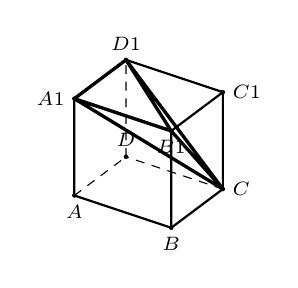
\begin{tikzpicture}[scale=0.82,line join=round,line cap=round]
  \coordinate (A) at (0,0);\coordinate (B) at (1.5,-0.5);\coordinate (D) at (0.8,0.6);\coordinate (C) at (2.3,0.1);
  \coordinate (A1) at (0,1.5);\coordinate (B1) at (1.5,1.0);\coordinate (D1) at (0.8,2.1);\coordinate (C1) at (2.3,1.6);
  \draw[dashed] (A)--(D) (C)--(D) (D)--(D1);
  \draw[thick] (A)--(B)--(C)--(C1)--(D1)--(A1)--cycle;
  \draw[thick] (A1)--(B1)--(C1) (B)--(B1);
  \draw[very thick] (A1)--(C) (A1)--(B1) (B1)--(C) (C)--(D1) (D1)--(A1) (B1)--(D1);
  \foreach \p/\pos in {A/below,B/below,C/right,D/above,A1/left,B1/below,C1/right,D1/above}{\fill (\p) circle (1pt) node[\pos]{\scriptsize\(\p\)};}
\end{tikzpicture}}
\answerblank[3.8cm]{解：}
\postproblem{
  \item 四个顶点本身都是正方体顶点，怎样用“补形”快速定位球心？
  \item 体积计算中，哪一个面作为底面能让高最容易看出来？
}{
  \checkbox 能识别补形模型\quad
  \checkbox 能把空间问题压缩到核心截面/长方体对角线
}{1.0cm}

\newpage

\subsection{专题四：解三角形中的“统一语言”}

\begin{theorembox}{正弦定理与余弦定理的选择}
\begin{center}
\begin{tabularx}{\textwidth}{p{3.4cm}p{3.0cm}X}
\toprule
\textbf{已知结构} & \textbf{优先工具} & \textbf{提醒}\\
\midrule
两角及一边 & 正弦定理 & 直接建立边角比例\\ \hline
两边及夹角 & 余弦定理 & 先求第三边或建立平方关系\\ \hline
三边或三边关系 & 余弦定理 & 常把目标角压缩为 $\cos A=k$\\ \hline
两边及其中一边对角 & 正弦定理 & 注意 SSA 情形可能有 $0/1/2$ 个三角形，必须检查角的可行性\\
\bottomrule
\end{tabularx}
\end{center}
\end{theorembox}

\sineLawFigure
\cosineLawFigure

\begin{decisionbox}{边角混合时，不要机械规定“永远化边”或“永远化角”}
\textbf{判断标准只有一个：哪种语言更接近目标状态。}
\begin{itemize}
  \item 若最终要用余弦定理锁定角，通常把正弦项先转为边更自然；
  \item 若目标是角的范围、和差或三角恒等式，统一成角可能更短；
  \item 若含面积，注意 $S=\tfrac12bc\sin A$ 可以在边与角之间充当“桥梁”。
\end{itemize}
\end{decisionbox}

\problemheader{经典训练四：边角互化与范围}
{\small 在 $\triangle ABC$ 中，已知 $2b\cos C=2a-c$，求角 $B$；若 $b=\sqrt3$，进一步研究三角形面积的最大值。}
\answerblank[4.2cm]{解：}
\postproblem{
  \item 第一问的目标状态可以预判成什么？
  \item 第二问要最大化面积，本质上需要控制哪一个乘积或三角函数量？
  \item 等号成立时，对应的三角形是否真实存在？
}{
  \checkbox 能根据目标选择“化边/化角”\quad
  \checkbox 会检验最值取等条件
}{1.0cm}

\newpage

\subsection{专题五：卷面表达——从“六步法”到最短完整证明链}

\begin{theorembox}{六个检查点}
\begin{enumerate}
  \item \textbf{设}：新变量、坐标系、参数对象是否定义清楚？
  \item \textbf{限}：定义域、换元范围、区间端点是否写出？
  \item \textbf{联}：关键方程来自哪个定理或几何关系？
  \item \textbf{推}：关键等价、推出、分类之间的逻辑方向是否清楚？
  \item \textbf{算}：判别式、韦达关系、导数符号等关键采分结果是否出现？
  \item \textbf{综}：最终结论是否回到题目原变量、原范围、原命题？
\end{enumerate}
\end{theorembox}

\begin{warningbox}{“六步”不是六段}
简单问题可能只需要其中三四项显式写出；复杂证明可能需要重复某些环节。它的作用是\textbf{检查逻辑闭环}，不是制造统一模板。
\end{warningbox}

\begin{theorembox}{两个高频书写细节}
\begin{itemize}
  \item \textbf{线面垂直判定}：若用“垂直于平面内两条相交直线”判定，必须把“两直线在平面内且相交”的条件写全。
  \item \textbf{单调区间表达}：多个单调区间应分别写出，用“在区间 $I_1$ 和 $I_2$ 上单调递增”表达；一般不要用并集符号把两个不相连区间伪装成一个区间。
\end{itemize}
\end{theorembox}

\newpage

% =====================================================
% 第五章 最终式思想
% =====================================================
\section{目标状态（最终式）思想：以终为始，但不“往答案上凑”}

\subsection{严格定义}
\begin{keybox}{什么叫“最终式”}
“最终式”是\textbf{足以直接推出题目目标的最低信息结构}。它不是预知答案，也不是为了配出标准答案而逆向凑式子，而是提前判断：\textbf{做到什么程度，问题就已经完成。}
\end{keybox}

实战中用以下五步：
\begin{enumerate}
  \item \textbf{读目标}：要角、边、比值、范围、定值、定点还是证明；
  \item \textbf{预测目标结构}：例如“求角”可能终止于 $\cos A=k$，“求范围”可能终止于一元函数 $f(t)$ 及其定义域；
  \item \textbf{选择桥梁}：决定正弦/余弦定理、韦达、向量、距离、换元等哪个工具最接近目标；
  \item \textbf{压缩链路}：优先保留能改变结构的关键步骤，不做没有目标的展开；
  \item \textbf{检验终止条件}：是否已经足够推出结论？是否仍缺范围、存在性或取等条件？
\end{enumerate}

\subsection{几个典型目标状态}
\begin{longtable}{p{3.2cm}p{5.4cm}p{6.5cm}}
\toprule
\textbf{题目目标} & \textbf{常见最终式} & \textbf{它暗示的路径}\\
\midrule
求角 & $\cos A=k$ / $\sin A=k$ & 统一边角、构造直角三角形、数量积\\ \hline
求参数范围 & $f(t)\ge0,\ t\in I$ & 降维 + 定义域 + 最值/判别式\\ \hline
求定值 & $E=\text{常数}$ 且动参消失 & 寻找对称式、韦达、齐次化、消元\\ \hline
定点/定直线 & 方程化为与动参无关的固定关系 & 分离参数、恒等系数、特殊位置猜测后证明\\ \hline
证明垂直 & $\vec a\cdot\vec b=0$ 或标准几何判定条件 & 建系/向量或寻找相交直线\\ \hline
证明存在 & 构造对象 + 验证全部约束 & 从目标反推构造，再正向验合法性\\
\bottomrule
\end{longtable}

\subsection{三角中的应用：最终式不是固定“纯边化”}
如果目标是求角 $A$，一种高频路线是
\[
\text{边角混合条件}
\longrightarrow \text{统一语言}
\longrightarrow \text{整理成 }b^2+c^2-a^2=\lambda bc
\longrightarrow \cos A=\frac\lambda2.
\]
但若原式本身已经高度三角化，强行纯边反而可能更长。\textbf{最终式决定语言，语言不应反过来绑架最终式。}

\subsection{解析几何中的应用：先知道要消掉谁}
定值、定点题运算量大，最危险的不是算错，而是\textbf{不知道为什么展开}。在联立前先写清：
\begin{itemize}
  \item 哪些是动参数？
  \item 最终哪些参数必须消失？
  \item 根与系数关系能否把两个交点压缩成对称式？
  \item 是否可以先分离常数，避免完整通分？
\end{itemize}

\begin{theorembox}{三个常用结构技巧}
\textbf{分离常数：}
\[
\frac{x-a}{x-b}=1+\frac{b-a}{x-b}.
\]
若同时含两个根 $x_1,x_2$，则后续往往只需处理
\[
\frac1{x_1-b}+\frac1{x_2-b},
\]
更容易接入韦达定理。

\medskip
\textbf{比值换元：}若目标本身是 $b/c$，且式子具有齐次性，可令 $t=b/c$，直接围绕目标降维。

\medskip
\textbf{整体目标换元：}若题目反复出现 $a-c$、$\alpha-\beta$ 等整体，不要急着拆开；把目标整体设为新变量，常能减少无效自由度。
\end{theorembox}

\newpage

% =====================================================
% 第六章 重复本
% =====================================================
\section{重复本系统：训练“路径召回”，而不是收藏错题}

\begin{keybox}{重复本的真正目标}
看到题目后，能够快速回答：\textbf{第一反应是什么？最终要做到什么结构？中间最关键的转化是什么？最大的合法性风险是什么？}
\end{keybox}

\subsection{一题只记录六个字段}
\begin{center}
\begin{tabularx}{0.96\textwidth}{p{2.6cm}X}
\toprule
\textbf{字段} & \textbf{填写内容}\\
\midrule
题目特征 & 不抄题干，写“边角混合 + 求角”“圆锥曲线两交点 + 定值”等结构标签\\ \hline
目标状态 & 做到什么式子即可结束，如 $\cos A=k$、消去动参、$f(t)\ge0$\\ \hline
第一反应 & 第一优先策略：定义域、统一边角、韦达、数形、分类……\\ \hline
关键转化 & 真正改变问题难度的那一步，而不是全部计算过程\\ \hline
失败信号 & 当时为什么卡住：过早展开、漏范围、选错表征、分类失控……\\ \hline
最终校验 & 端点、等号、增漏解、几何存在性、原变量回代\\
\bottomrule
\end{tabularx}
\end{center}

\subsection{三轮训练，而不是“重抄三遍”}
\begin{enumerate}
  \item \textbf{第一轮：完整解决。}允许看解析，但必须标出关键转化和错误来源；
  \item \textbf{第二轮：只看题目复述路径。}暂不计算，先说出目标状态、第一反应和两三个关键节点；
  \item \textbf{第三轮：限时重建。}完整独立解答，并比较是否比第一次路径更短、更稳。
\end{enumerate}

\begin{trainingbox}{真正“掌握”的判据}
不是“答案我看懂了”，而是隔一段时间重新看到题目时，能在开始大量计算前恢复出大致的结构链：
\[
\text{题目特征}\rightarrow\text{目标状态}\rightarrow\text{关键转化}\rightarrow\text{验证点}.
\]
\end{trainingbox}

\subsection{重复本选题标准}
优先收录：
\begin{enumerate}
  \item 包装陌生，但拆开后是高频结构；
  \item 方法知道，第一反应却慢；
  \item 运算链较长，且某一步有明显结构技巧；
  \item 同一种错误已经重复出现；
  \item 一题可以代表一整类“触发信号 $\rightarrow$ 决策”的母题。
\end{enumerate}

\newpage

% =====================================================
% 第七章 考场流程
% =====================================================
\section{考场卡壳时的救援流程：不是一直往前冲，而是允许回退}

\begin{center}
\resizebox{0.96\textwidth}{!}{%
\begin{tikzpicture}[
  node distance=1.0cm and 1.4cm,
  every node/.style={draw,thick,rectangle,rounded corners=4pt,align=center,inner sep=7pt,fill=white,font=\small},
  arrow/.style={-{Latex[length=2.2mm]},thick}
]
  \node (goal) [text width=7.5cm] {\textbf{1. 读目标}\quad 最终需要角、边、范围、定值、存在性还是证明？\\先写出“做到什么就够了”};
  \node (constraint) [below=of goal,text width=7.5cm] {\textbf{2. 扫约束}\quad 定义域、非零、参数范围、几何存在性、换元范围};
  \node (repr) [below=of constraint,text width=7.5cm] {\textbf{3. 选表征}\quad 函数 / 方程 / 图像 / 几何 / 向量，哪种语言最接近目标？};
  \node (path) [below=of repr,text width=7.5cm] {\textbf{4. 搜路径}\quad 正推？逆推？分类？特殊值？换元？数形？};
  \node (calc) [below left=1.3cm and 0.0cm of path,text width=5.0cm] {\textbf{5. 执行关键转化}\\降维、消元、整体化、对称化\\只做有目标的计算};
  \node (fail) [below right=1.3cm and 0.0cm of path,text width=5.0cm] {\textbf{失败信号}\\越算变量越多 / 展开失控 / 目标越来越远};
  \node (verify) [below=4.0cm of path,text width=7.5cm] {\textbf{6. 验证}\quad 端点、等号、增漏解、原题回代、实际存在性};
  \node (write) [below=of verify,text width=7.5cm] {\textbf{7. 写闭环}\quad 用最短完整逻辑链呈现关键依据与结论};

  \draw[arrow] (goal)--(constraint);
  \draw[arrow] (constraint)--(repr);
  \draw[arrow] (repr)--(path);
  \draw[arrow] (path)--(calc);
  \draw[arrow] (path)--(fail);
  \draw[arrow] (calc)|-(verify);
  \draw[arrow] (fail.east) -- ++(1.4,0) |- node[pos=0.3,right,draw=none]{回退} (repr.east);
  \draw[arrow] (verify)--(write);
\end{tikzpicture}}
\end{center}

\begin{keybox}{考场原则：先控制方向，再提高速度}
真正浪费时间的往往不是某一步算慢，而是在错误表征上高速计算。卡壳时最有价值的问题不是“我还能算什么”，而是：\textbf{我是不是正在用错误的语言描述这道题？}
\end{keybox}

\newpage

% =====================================================
% 第八章 自检清单
% =====================================================
\section{一页自检：做完一道题后，只问这 10 个问题}

\begin{enumerate}
  \item 我能一句话说出这道题真正考的\textbf{结构}，而不只是章节名称吗？
  \item 我知道这道题的\textbf{最终式/目标状态}是什么吗？
  \item 第一条路线为什么值得尝试？它的\textbf{触发信号}是什么？
  \item 有没有更自然的表征：函数、图像、几何、向量？
  \item 我写清楚所有定义域、换元范围和非零条件了吗？
  \item 哪一步只是“推出”，哪一步真正“等价”？
  \item 是否存在边界、端点、等号成立条件需要回代？
  \item 如果我走错路，最早在哪一步应该发现？
  \item 我的卷面是否包含关键依据，又没有无效废话？
  \item 一周以后再看这道题，我希望自己记住的是哪一个\textbf{结构链}？
\end{enumerate}

\begin{trainingbox}{最后一句}
不要把“做过”当成“会做”，也不要把“会算”当成“会解题”。真正稳定的能力，是陌生包装改变以后，你仍然能完成：
\[
\boxed{\text{识别结构}\rightarrow\text{预测目标}\rightarrow\text{选择转化}\rightarrow\text{控制合法性}\rightarrow\text{验证边界}}.
\]
\end{trainingbox}

\vfill
\begin{center}
\rule{0.7\textwidth}{0.5pt}\\[0.5em]
\small 本手册以“问题解决控制系统”为主线；具体题型、真题与专题技巧均作为可挂载训练模块。\par
\end{center}

\end{document}
